% ======================================================================
\section{Shortest paths and the cost of induced bonds}\label{sec:paths}
% ======================================================================

This section shows that the weight of a shortest path decays exponentially in its length, up to a price paid for each chord (\cref{prop:cost}). The argument has four steps. A shortest path in a high-temperature graph forbids all bonds spanned by its vertices (\cref{lem:selection}). The cost of removing these bonds is a sum of correlation integrals (\cref{lem:interp}). Each integral is bounded below on a fixed $28$-site graph (\cref{lem:prismbound,cert:prism}). Finally the integrals are redistributed to the vertices of the path (\cref{def:allocation,cert:allocation}).

Throughout \cref{sec:paths,sec:counting,sec:lower}, $L\ge8$ is even and $G_L(x,y)=\avg{\sigma_x\sigma_y}_{L,K}$ denotes the zero-field periodic two-point function.

\subsection{Selected paths}

A \emph{path} $P=(v_0,v_1,\dots,v_n)$ of length $|P|=n\ge1$ on $\T_L$ is a sequence of distinct sites with $v_{i-1}\sim v_i$ for all $i$. Its vertex set is $V(P)$ and its bond set is $E(P)=\{\{v_{i-1},v_i\}:1\le i\le n\}$. We write $\cS_{xy}$ for the set of paths from $x$ to $y$.

\begin{definition}[Induced bonds and chords]\label{def:induced}
The \emph{induced bond set} of $P$ is $D(P)=\{\{x,y\}\in E_L:\ x,y\in V(P)\}$. Its elements outside $E(P)$ are the \emph{chords} of $P$, and $c(P)=|D(P)|-|P|$ is the \emph{chord number}. A chord joins two nonconsecutive vertices of $P$. Chords across the periodic identification are included.
\end{definition}

\begin{lemma}[Selection of a shortest path]\label{lem:selection}
For $x\ne y$ in $\T_L$,
\begin{equation}\label{eq:selection}
 G_L(x,y)\le\sum_{P\in\cS_{xy}}u^{|P|}\,e^{-I(P,u)},\qquad
 I(P,u)=\log\frac{\cE(u)}{\cE(u\one_{E_L\setminus D(P)})}\ \ge0 .
\end{equation}
\end{lemma}

\begin{proof}
By~\eqref{eq:HT}, $G_L(x,y)=\cE(u)^{-1}\sum_Au^{|A|}$, where $A$ ranges over two-source bond sets with $\partial A=\{x,y\}$. Every such $A$ contains a path from $x$ to $y$. Fix a total order on $\cS_{xy}$ and let $P(A)$ be the first among the shortest such paths contained in $A$. If a chord $\{v_i,v_j\}$, $j>i+1$, of $P(A)$ belonged to $A$, then $(v_0,\dots,v_i,v_j,\dots,v_n)$ would be a strictly shorter path in $A$. Hence $A\cap D(P(A))=E(P(A))$. The set $B=A\setminus E(P(A))$ is even, because deleting a path changes the parity of degrees only at its endpoints, and $B\subset E_L\setminus D(P(A))$. The map $A\mapsto(P(A),B)$ is injective since $A=E(P(A))\cup B$. Therefore
\[
 \sum_Au^{|A|}\le\sum_{P\in\cS_{xy}}u^{|P|}\sum_{\substack{B\subset E_L\setminus D(P)\\ \partial B=\varnothing}}u^{|B|}
 =\sum_{P\in\cS_{xy}}u^{|P|}\,\cE(u\one_{E_L\setminus D(P)}).
\]
Dividing by $\cE(u)$ gives~\eqref{eq:selection}. Finally $I(P,u)\ge0$ because $\cE$ has nonnegative coefficients.
\end{proof}

Fisher's bound~\cite{Fis67} is the special case in which the factor $e^{-I(P,u)}$ is dropped. The rest of this section bounds $I(P,u)$ from below.

\subsection{Interpolation}

Fix $P$ and write $D=D(P)$. For $s\in[0,u]$ let $a^{(s)}\in[0,1)^{E_L}$ be the bond weights
\[
 a^{(s)}_f=s\quad(f\in D),\qquad a^{(s)}_f=u\quad(f\notin D).
\]
For $e=\{v,w\}\in D$ let $C_e(s)=\avg{\sigma_v\sigma_w}_{\T_L-e,\,a^{(s)}}$ be the correlation across $e$ in the interpolated model with $e$ removed.

\begin{lemma}[Interpolation identity]\label{lem:interp}
\begin{equation}\label{eq:interp}
 I(P,u)=\sum_{e\in D(P)}\int_0^u\frac{C_e(s)}{1+sC_e(s)}\,\dd s .
\end{equation}
\end{lemma}

\begin{proof}
Let $\phi(s)=\log\cE_{\T_L}(a^{(s)})$. Then $\phi(u)=\log\cE(u)$ and $\phi(0)=\log\cE(u\one_{E_L\setminus D})$, so $I(P,u)=\phi(u)-\phi(0)$. By the chain rule, $\phi'(s)=\sum_{e\in D}\partial_{a_e}\log\cE(a)|_{a=a^{(s)}}$, and \cref{lem:factor} identifies each term with $C_e(s)/(1+sC_e(s))$.
\end{proof}

All terms in~\eqref{eq:interp} refer to the \emph{same} interpolated system. They can therefore be estimated independently, and the auxiliary graphs used for different bonds may overlap. By \cref{lem:factor} and the remark after it we obtain the following.

\begin{corollary}[Local comparison]\label{cor:local}
Let $e=\{v,w\}\in D(P)$, let $\Gamma$ be a subgraph of $\T_L-e$ containing $v,w$, and let $b$ be bond weights on $\Gamma$ with $0\le b_f\le a^{(s)}_f$ for every bond $f$ of $\Gamma$. Then $C_e(s)\ge\avg{\sigma_v\sigma_w}_{\Gamma,b}$, and the integrand in~\eqref{eq:interp} is at least $\avg{\sigma_v\sigma_w}_{\Gamma,b}/(1+s\avg{\sigma_v\sigma_w}_{\Gamma,b})$.
\end{corollary}

\subsection{The prism}

Let $e=\{v,w\}$ be a bond of $\T_L$ with $w=v+\delta$, $\delta$ a unit vector, which we call the \emph{axial} direction of $e$. Let $\pm\epsilon_1,\pm\epsilon_2$ be the four unit vectors orthogonal to $\delta$, the \emph{transverse} directions. The two endpoints $v,w$ are the \emph{hubs} of $e$.

\begin{definition}[Prism]\label{def:prism}
The \emph{prism} of $e$ is the induced subgraph of $\T_L$ on the $28$ sites
\[
 \Pi(e)=\{v+t\delta+y\epsilon_1+z\epsilon_2:\ t\in\{0,1\},\ |y|,|z|\le1\}\ \cup\
 \{v+t\delta+y\epsilon_1+z\epsilon_2:\ t\in\{-1,2\},\ |y|+|z|\le1\},
\]
with the bond $e$ removed. It has $51-1=50$ bonds (\cref{fig:prism}). Since $L\ge8$, the sites are distinct and the bonds are those of $\Z^3$.
\end{definition}

Ten sites of $\Pi(e)$ are adjacent to a hub: the four transverse neighbours $v\pm\epsilon_i$ and the opposite axial neighbour $v-\delta$ of $v$, and likewise $w\pm\epsilon_i$ and $w+\delta$. These are the \emph{specified sites}. The other $16$ sites are the eight corners of the two $3\times3$ squares and the eight transverse arms of the two end crosses.

\begin{definition}[Pattern]\label{def:pattern}
Let $P$ be a path and $e\in D(P)$ with hubs $v,w$. The \emph{pattern} $h(e)$ consists of the ten indicators $\one\{x\in V(P)\}$ of the specified sites. We write it as $h=(\mathbf a,o;\mathbf a',o')$, where $\mathbf a\in\{0,1\}^4$ records the transverse neighbours of $v$, $o$ the opposite axial neighbour of $v$, and $\mathbf a',o'$ the same at $w$. There are $2^{10}=1024$ patterns.
\end{definition}

\begin{figure}[t]
\centering
\begin{tikzpicture}[scale=1.2,line cap=round]
\draw[black!45,line width=0.55pt] (0.620,-0.600) -- (0.620,0.400);
\draw[black!45,line width=0.55pt] (0.620,-0.600) -- (2.670,-0.600);
\draw[black!45,line width=0.55pt] (0.620,0.400) -- (0.620,1.400);
\draw[black!45,line width=0.55pt] (0.620,0.400) -- (2.670,0.400);
\draw[black!45,line width=0.55pt] (0.620,0.400) -- (-1.430,0.400);
\draw[black!45,line width=0.55pt] (0.620,1.400) -- (2.670,1.400);
\draw[black!45,line width=0.55pt] (2.670,-0.600) -- (2.670,0.400);
\draw[black!45,line width=0.55pt] (2.670,0.400) -- (2.670,1.400);
\draw[black!45,line width=0.55pt] (2.670,0.400) -- (4.720,0.400);
\draw[black!45,line width=0.55pt] (0.000,-1.000) -- (0.620,-0.600);
\draw[black!45,line width=0.55pt] (0.000,0.000) -- (0.620,0.400);
\draw[black!45,line width=0.55pt] (0.000,1.000) -- (0.620,1.400);
\draw[black!45,line width=0.55pt] (2.050,-1.000) -- (2.670,-0.600);
\draw[black!45,line width=0.55pt] (2.050,0.000) -- (2.670,0.400);
\draw[black!45,line width=0.55pt] (2.050,1.000) -- (2.670,1.400);
\draw[black!45,line width=0.55pt] (-2.050,0.000) -- (-1.430,0.400);
\draw[black!45,line width=0.55pt] (4.100,0.000) -- (4.720,0.400);
\draw[black!45,line width=0.55pt] (0.000,-1.000) -- (0.000,0.000);
\draw[black!45,line width=0.55pt] (0.000,-1.000) -- (2.050,-1.000);
\draw[black!45,line width=0.55pt] (0.000,-1.000) -- (-2.050,-1.000);
\draw[black!45,line width=0.55pt] (0.000,0.000) -- (0.000,1.000);
\draw[black!45,line width=0.55pt] (0.000,0.000) -- (-2.050,0.000);
\draw[black!45,line width=0.55pt] (0.000,1.000) -- (2.050,1.000);
\draw[black!45,line width=0.55pt] (0.000,1.000) -- (-2.050,1.000);
\draw[black!45,line width=0.55pt] (2.050,-1.000) -- (2.050,0.000);
\draw[black!45,line width=0.55pt] (2.050,-1.000) -- (4.100,-1.000);
\draw[black!45,line width=0.55pt] (2.050,0.000) -- (2.050,1.000);
\draw[black!45,line width=0.55pt] (2.050,0.000) -- (4.100,0.000);
\draw[black!45,line width=0.55pt] (2.050,1.000) -- (4.100,1.000);
\draw[black!45,line width=0.55pt] (-2.050,0.000) -- (-2.050,1.000);
\draw[black!45,line width=0.55pt] (-2.050,0.000) -- (-2.050,-1.000);
\draw[black!45,line width=0.55pt] (4.100,0.000) -- (4.100,1.000);
\draw[black!45,line width=0.55pt] (4.100,0.000) -- (4.100,-1.000);
\draw[black!45,line width=0.55pt] (-0.620,-1.400) -- (0.000,-1.000);
\draw[black!45,line width=0.55pt] (-0.620,-0.400) -- (0.000,0.000);
\draw[black!45,line width=0.55pt] (-0.620,0.600) -- (0.000,1.000);
\draw[black!45,line width=0.55pt] (1.430,-1.400) -- (2.050,-1.000);
\draw[black!45,line width=0.55pt] (1.430,-0.400) -- (2.050,0.000);
\draw[black!45,line width=0.55pt] (1.430,0.600) -- (2.050,1.000);
\draw[black!45,line width=0.55pt] (-2.050,0.000) -- (-2.670,-0.400);
\draw[black!45,line width=0.55pt] (4.100,0.000) -- (3.480,-0.400);
\draw[black!45,line width=0.55pt] (-0.620,-1.400) -- (-0.620,-0.400);
\draw[black!45,line width=0.55pt] (-0.620,-1.400) -- (1.430,-1.400);
\draw[black!45,line width=0.55pt] (-0.620,-0.400) -- (-0.620,0.600);
\draw[black!45,line width=0.55pt] (-0.620,-0.400) -- (1.430,-0.400);
\draw[black!45,line width=0.55pt] (-0.620,-0.400) -- (-2.670,-0.400);
\draw[black!45,line width=0.55pt] (-0.620,0.600) -- (1.430,0.600);
\draw[black!45,line width=0.55pt] (1.430,-1.400) -- (1.430,-0.400);
\draw[black!45,line width=0.55pt] (1.430,-0.400) -- (1.430,0.600);
\draw[black!45,line width=0.55pt] (1.430,-0.400) -- (3.480,-0.400);
\draw[red!70!black,line width=1.4pt,dash pattern=on 3pt off 2pt] (0.000,0.000) -- (2.050,0.000);
\filldraw[fill=black!35,draw=black!60,line width=0.5pt] (0.620,-0.600) circle (2.6pt);
\filldraw[fill=black!35,draw=black!60,line width=0.5pt] (2.670,-0.600) circle (2.6pt);
\filldraw[fill=white,draw=black,line width=0.9pt] (0.620,0.400) circle (3.2pt);
\filldraw[fill=white,draw=black,line width=0.9pt] (2.670,0.400) circle (3.2pt);
\filldraw[fill=black!35,draw=black!60,line width=0.5pt] (4.720,0.400) circle (2.6pt);
\filldraw[fill=black!35,draw=black!60,line width=0.5pt] (-1.430,0.400) circle (2.6pt);
\filldraw[fill=black!35,draw=black!60,line width=0.5pt] (0.620,1.400) circle (2.6pt);
\filldraw[fill=black!35,draw=black!60,line width=0.5pt] (2.670,1.400) circle (2.6pt);
\filldraw[fill=white,draw=black,line width=0.9pt] (0.000,1.000) circle (3.2pt);
\filldraw[fill=black!35,draw=black!60,line width=0.5pt] (4.100,1.000) circle (2.6pt);
\filldraw[fill=white,draw=black,line width=0.9pt] (2.050,1.000) circle (3.2pt);
\filldraw[fill=white,draw=black,line width=0.9pt] (0.000,-1.000) circle (3.2pt);
\filldraw[fill=black!35,draw=black!60,line width=0.5pt] (-2.050,1.000) circle (2.6pt);
\filldraw[fill=white,draw=black,line width=0.9pt] (2.050,-1.000) circle (3.2pt);
\filldraw[fill=black!35,draw=black!60,line width=0.5pt] (4.100,-1.000) circle (2.6pt);
\fill[black] (0.000,0.000) circle (3.6pt);
\fill[black] (2.050,0.000) circle (3.6pt);
\filldraw[fill=white,draw=black,line width=0.9pt] (4.100,0.000) circle (3.2pt);
\filldraw[fill=black!35,draw=black!60,line width=0.5pt] (-2.050,-1.000) circle (2.6pt);
\filldraw[fill=white,draw=black,line width=0.9pt] (-2.050,0.000) circle (3.2pt);
\filldraw[fill=black!35,draw=black!60,line width=0.5pt] (-0.620,-1.400) circle (2.6pt);
\filldraw[fill=black!35,draw=black!60,line width=0.5pt] (1.430,-1.400) circle (2.6pt);
\filldraw[fill=white,draw=black,line width=0.9pt] (-0.620,-0.400) circle (3.2pt);
\filldraw[fill=white,draw=black,line width=0.9pt] (1.430,-0.400) circle (3.2pt);
\filldraw[fill=black!35,draw=black!60,line width=0.5pt] (3.480,-0.400) circle (2.6pt);
\filldraw[fill=black!35,draw=black!60,line width=0.5pt] (-2.670,-0.400) circle (2.6pt);
\filldraw[fill=black!35,draw=black!60,line width=0.5pt] (-0.620,0.600) circle (2.6pt);
\filldraw[fill=black!35,draw=black!60,line width=0.5pt] (1.430,0.600) circle (2.6pt);
\node[below left=1pt] at (0.000,0.000) {$v$};
\node[below right=1pt] at (2.050,0.000) {$w$};
\node[red!70!black,above] at (1.025,0.000) {$e$};
\draw[-{Stealth[length=4pt]},thick] (-3.600,-2.300) -- ++(0.9,0) node[right] {$\delta$};
\draw[-{Stealth[length=4pt]},thick] (-3.600,-2.300) -- ++(0,0.75) node[above] {$\epsilon_1$};
\draw[-{Stealth[length=4pt]},thick] (-3.600,-2.300) -- ++(0.50,0.33) node[above right=-2pt] {$\epsilon_2$};
\node[font=\footnotesize,black!70] at (-2.050,-1.75) {$t=-1$};
\node[font=\footnotesize,black!70] at (0.000,-1.75) {$t=0$};
\node[font=\footnotesize,black!70] at (2.050,-1.75) {$t=1$};
\node[font=\footnotesize,black!70] at (4.100,-1.75) {$t=2$};
\fill[black] (5.6,1.1) circle (3.6pt) node[right=5pt,font=\small] {hubs};
\filldraw[fill=white,draw=black,line width=0.9pt] (5.6,0.55) circle (3.2pt) node[right=5pt,font=\small] {specified (label $h$)};
\filldraw[fill=black!35,draw=black!60] (5.6,0.0) circle (2.6pt) node[right=5pt,font=\small] {mark $1$};
\draw[red!70!black,line width=1.4pt,dash pattern=on 3pt off 2pt] (5.3999999999999995,-0.5499999999999998) -- (5.8,-0.5499999999999998) node[right=3pt,font=\small,black] {removed bond};
\end{tikzpicture}
\caption{The prism $\Pi(e)$ of \cref{def:prism}: two $3\times3$ squares at axial coordinates $t=0,1$ and two crosses at $t=-1,2$, with all $51$ lattice bonds among the $28$ sites except $e$. The label $h(e)$ records which of the ten specified sites belong to the path. The remaining $16$ sites are treated as occupied. Bonds between two sites of mark $1$ carry the interpolation weight $s$, all other bonds the reference weight $u_0$.}
\label{fig:prism}
\end{figure}


Fix a \emph{reference weight} $u_0\in(0,1)$. For a pattern $h$ assign a \emph{mark} $m(x)\in\{0,1\}$ to each site of $\Pi(e)$. The hubs get mark $1$. A specified site gets the indicator recorded in $h$. The $16$ other sites get mark $1$. For $s\in[0,u_0]$ give the bond $f=\{x,x'\}$ of $\Pi(e)$ the weight
\begin{equation}\label{eq:prismweights}
 b^{h,s}_f=s\ \text{ if } m(x)=m(x')=1,\qquad b^{h,s}_f=u_0\ \text{ otherwise}.
\end{equation}
Let $N_h(s)$ and $E_h(s)$ be the two-source polynomial $\cO_{\Pi(e)}(v,w;b^{h,s})$ and the even polynomial $\cE_{\Pi(e)}(b^{h,s})$. They are polynomials in $s$ with nonnegative rational coefficients when $u_0\in\mathbb Q$. They depend only on $h$ and $u_0$, not on $e$ or $L$. Define
\begin{equation}\label{eq:ellh}
 \ell_h(u_0)=\int_0^{u_0}\frac{N_h(s)}{E_h(s)+sN_h(s)}\,\dd s .
\end{equation}

\begin{lemma}[Local lower bound]\label{lem:prismbound}
Let $u\ge u_0$. For every path $P$ on $\T_L$,
\[
 I(P,u)\ \ge\ \sum_{e\in D(P)}\ell_{h(e)}(u_0).
\]
\end{lemma}

\begin{proof}
Fix $e\in D(P)$ and $s\in[0,u_0]$. We claim $b^{h(e),s}_f\le a^{(s)}_f$ for every bond $f=\{x,x'\}$ of $\Pi(e)$. If $f\in D(P)$, then $x,x'\in V(P)$. The marks dominate the true indicators of $V(P)$: the marks of hubs and specified sites are the true indicators, and the remaining sites have mark $1$. Hence $m(x)=m(x')=1$ and $b_f=s=a^{(s)}_f$. If $f\notin D(P)$, then $a^{(s)}_f=u\ge u_0\ge b_f$. By \cref{cor:local} with $\Gamma=\Pi(e)$ and~\eqref{eq:HT}, the integrand in~\eqref{eq:interp} is at least $N_h(s)/(E_h(s)+sN_h(s))$ for $s\le u_0$. The integrand is nonnegative on $[u_0,u]$, so the integral over $[0,u]$ is at least $\ell_{h(e)}(u_0)$. Summing over $e\in D(P)$ and using \cref{lem:interp} gives the claim.
\end{proof}

The rule ``unknown sites are occupied'' covers every possible continuation of the path outside the ten specified sites, including returns of the path into the prism, without enumerating them. The price is a pessimistic prism integral. Because $\ell_h(u_0)$ does not depend on $u\ge u_0$, a certificate computed at $u_0$ applies to every stronger coupling.

\begin{lemma}[Panel quadrature]\label{lem:panel}
For $0\le\alpha<\beta$,
\[
 \int_\alpha^\beta\frac{N_h(s)}{E_h(s)+sN_h(s)}\,\dd s\ \ge\ (\beta-\alpha)\,\frac{N_h\bigl(\tfrac{\alpha+\beta}2\bigr)}{E_h(\beta)+\beta N_h(\beta)} .
\]
\end{lemma}

\begin{proof}
The denominator has nonnegative coefficients, so it is nondecreasing on $[0,\infty)$ and bounded above by its value at $\beta$. The numerator has nonnegative coefficients and is therefore convex on $[0,\infty)$. Its mean over $[\alpha,\beta]$ is at least its value at the midpoint (Jensen).
\end{proof}

\begin{certificate}[Prism integrals]\label{cert:prism}
Let $u_0$ be one of the two reference weights
\[
 u_*=\frac{10829}{50829}\ \ (r_*=\tfrac{30829}{20000}),\qquad u_2=\frac{677}{3177}\ \ (r_2=\tfrac{1927}{1250}).
\]
Split $[0,u_0]$ into $64$ equal panels. For every pattern $h$ and every panel, the right-hand side of \cref{lem:panel} is evaluated exactly, multiplied by $10^{12}$ and rounded down to an integer. The sum of these $64$ integers, divided by $10^{12}$, is a rational number $\underline\ell_h(u_0)\le\ell_h(u_0)$. The $1024$ patterns fall into $123$ orbits under the symmetries of the transverse square and the exchange of the two hubs. The tables $(\underline\ell_h(u_*))_h$ and $(\underline\ell_h(u_2))_h$ are the input to \cref{cert:allocation}.
\end{certificate}

To give an idea of the size of these numbers, at $u_0=u_*$ the pattern of a straight bond with no transverse neighbours and both axial neighbours occupied ($\mathbf a=\mathbf a'=0$, $o=o'=1$) has $\underline\ell_h=0.010880485789$. The fully occupied pattern has $\underline\ell_h=0.002731285336$. The corresponding upper sums, with midpoint and right endpoint replaced by the trapezoid and the left endpoint, differ by less than $10^{-5}$. The local cost of an induced bond thus decreases by a factor of about four as its neighbourhood fills up. This is the effect that the allocation below has to control.

\subsection{Half-edge charges}

We now redistribute the integrals $\underline\ell_{h(e)}$ to the vertices of $P$. The scheme is a discharging argument. Each induced bond splits its prism integral between its two endpoints according to a fixed table, and the table is chosen so that every interior vertex of the path collects at least $\gamma$, whatever its occupied neighbourhood. A chord may hand out slightly more than its integral, and the excess is charged to the chord price $\theta$. Path bonds may in addition keep a shape charge $w_\tau$, which is summed separately in \cref{sec:counting}. For $e\in D(P)$ with endpoint $v$, let $\delta$ be the direction from $v$ to the other endpoint. The \emph{type} of the half-edge $(e,v)$ is
\begin{equation}\label{eq:type}
 t_v(e)=j+5o\in\{0,\dots,9\},\qquad j=\#\{\epsilon\perp\delta:\ v+\epsilon\in V(P)\},\quad o=\one\{v-\delta\in V(P)\}.
\end{equation}
The \emph{role} of $e$ is \emph{path} if $e\in E(P)$ and \emph{chord} otherwise. The type of each half-edge of $e$ is a function of the pattern $h(e)$.

\begin{definition}[Shapes]\label{def:shape}
Let $P=(v_0,\dots,v_n)$ and $1\le i\le n-2$. Put $\delta=v_{i+1}-v_i$, $d_-=v_{i-1}-v_i$ and $d_+=v_{i+2}-v_{i+1}$. Then $d_-\ne\delta$ and $d_+\ne-\delta$. The \emph{shape} $\tau_i$ of the triple $(v_{i-1}v_i,v_iv_{i+1},v_{i+1}v_{i+2})$ is
\begin{center}
\begin{tabular}{ll}
 $\mathrm S$ (straight) & $d_-=-\delta$ and $d_+=\delta$;\\
 $\mathrm A$ (one axial) & exactly one of $d_-=-\delta$, $d_+=\delta$ holds;\\
 $\mathrm U$ (equal transverse) & $d_\pm\perp\delta$ and $d_-=d_+$;\\
 $\mathrm T$ (perpendicular transverse) & $d_\pm\perp\delta$ and $d_-\perp d_+$;\\
 $\mathrm Z$ (opposite transverse) & $d_\pm\perp\delta$ and $d_-=-d_+$.
\end{tabular}
\end{center}
See \cref{fig:shapes}. In shape $\mathrm U$ the outer vertices $v_{i-1},v_{i+2}$ are adjacent and span a chord.
\end{definition}

\begin{figure}[t]
\centering
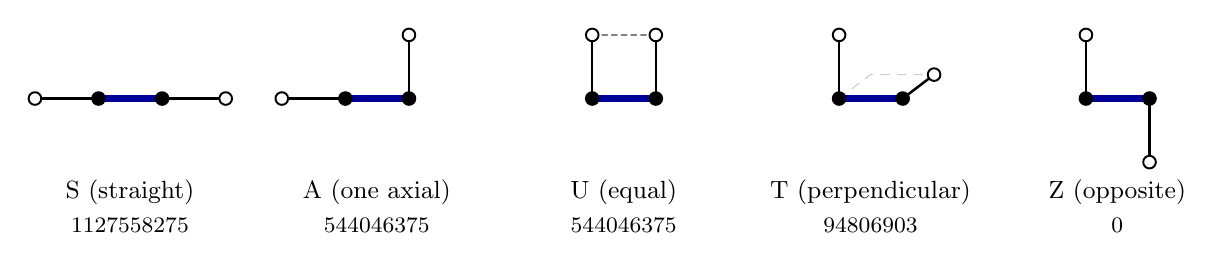
\begin{tikzpicture}[scale=0.95,line cap=round,line join=round]
\draw[black,line width=0.9pt] (-0.850,0.000) -- (0.000,0.000);
\draw[black,line width=0.9pt] (0.850,0.000) -- (1.700,0.000);
\draw[blue!60!black,line width=2.2pt] (0.000,0.000) -- (0.850,0.000);
\filldraw[fill=white,draw=black,line width=0.7pt] (-0.850,0.000) circle (2.4pt);
\filldraw[fill=black,draw=black,line width=0.7pt] (0.000,0.000) circle (2.4pt);
\filldraw[fill=black,draw=black,line width=0.7pt] (0.850,0.000) circle (2.4pt);
\filldraw[fill=white,draw=black,line width=0.7pt] (1.700,0.000) circle (2.4pt);
\node[font=\small] at (0.420,-1.25) {$\mathrm{S}$ (straight)};
\node[font=\footnotesize] at (0.420,-1.7) {$1127558275$};
\draw[black,line width=0.9pt] (2.450,0.000) -- (3.300,0.000);
\draw[black,line width=0.9pt] (4.150,0.000) -- (4.150,0.850);
\draw[blue!60!black,line width=2.2pt] (3.300,0.000) -- (4.150,0.000);
\filldraw[fill=white,draw=black,line width=0.7pt] (2.450,0.000) circle (2.4pt);
\filldraw[fill=black,draw=black,line width=0.7pt] (3.300,0.000) circle (2.4pt);
\filldraw[fill=black,draw=black,line width=0.7pt] (4.150,0.000) circle (2.4pt);
\filldraw[fill=white,draw=black,line width=0.7pt] (4.150,0.850) circle (2.4pt);
\node[font=\small] at (3.720,-1.25) {$\mathrm{A}$ (one axial)};
\node[font=\footnotesize] at (3.720,-1.7) {$544046375$};
\draw[black!50,dash pattern=on 2pt off 1.5pt] (6.600,0.850) -- (7.450,0.850);
\draw[black,line width=0.9pt] (6.600,0.850) -- (6.600,0.000);
\draw[black,line width=0.9pt] (7.450,0.000) -- (7.450,0.850);
\draw[blue!60!black,line width=2.2pt] (6.600,0.000) -- (7.450,0.000);
\filldraw[fill=white,draw=black,line width=0.7pt] (6.600,0.850) circle (2.4pt);
\filldraw[fill=black,draw=black,line width=0.7pt] (6.600,0.000) circle (2.4pt);
\filldraw[fill=black,draw=black,line width=0.7pt] (7.450,0.000) circle (2.4pt);
\filldraw[fill=white,draw=black,line width=0.7pt] (7.450,0.850) circle (2.4pt);
\node[font=\small] at (7.020,-1.25) {$\mathrm{U}$ (equal)};
\node[font=\footnotesize] at (7.020,-1.7) {$544046375$};
\draw[black!20,dashed] (9.900,0.000) -- (10.320,0.320) -- (11.170,0.320);
\draw[black,line width=0.9pt] (9.900,0.850) -- (9.900,0.000);
\draw[black,line width=0.9pt] (10.750,0.000) -- (11.170,0.320);
\draw[blue!60!black,line width=2.2pt] (9.900,0.000) -- (10.750,0.000);
\filldraw[fill=white,draw=black,line width=0.7pt] (9.900,0.850) circle (2.4pt);
\filldraw[fill=black,draw=black,line width=0.7pt] (9.900,0.000) circle (2.4pt);
\filldraw[fill=black,draw=black,line width=0.7pt] (10.750,0.000) circle (2.4pt);
\filldraw[fill=white,draw=black,line width=0.7pt] (11.170,0.320) circle (2.4pt);
\node[font=\small] at (10.320,-1.25) {$\mathrm{T}$ (perpendicular)};
\node[font=\footnotesize] at (10.320,-1.7) {$94806903$};
\draw[black,line width=0.9pt] (13.200,0.850) -- (13.200,0.000);
\draw[black,line width=0.9pt] (14.050,0.000) -- (14.050,-0.850);
\draw[blue!60!black,line width=2.2pt] (13.200,0.000) -- (14.050,0.000);
\filldraw[fill=white,draw=black,line width=0.7pt] (13.200,0.850) circle (2.4pt);
\filldraw[fill=black,draw=black,line width=0.7pt] (13.200,0.000) circle (2.4pt);
\filldraw[fill=black,draw=black,line width=0.7pt] (14.050,0.000) circle (2.4pt);
\filldraw[fill=white,draw=black,line width=0.7pt] (14.050,-0.850) circle (2.4pt);
\node[font=\small] at (13.620,-1.25) {$\mathrm{Z}$ (opposite)};
\node[font=\footnotesize] at (13.620,-1.7) {$0$};
\end{tikzpicture}
\caption{The five shapes of a triple of consecutive path bonds (\cref{def:shape}). The middle bond, whose endpoints are the two hubs, is drawn thick. The numbers are the shape charges $10^{12}w_\tau$ of \cref{tab:shapes}. In shape $\mathrm U$ the two outer vertices span a chord (dashed).}
\label{fig:shapes}
\end{figure}


\begin{definition}[Admissible allocation]\label{def:allocation}
Let $\ell=(\ell_h)_h$ be a table of $1024$ nonnegative numbers. An \emph{allocation} consists of path charges $\alpha^{\rm P}_t\ge0$ and chord charges $\alpha^{\rm C}_t\ge0$ for $t=0,\dots,9$, shape charges $w_\tau\ge0$ for $\tau\in\{\mathrm S,\mathrm A,\mathrm U,\mathrm T,\mathrm Z\}$, a chord price $\theta\ge0$ and a vertex gain $\gamma$. It is \emph{admissible for $\ell$} if the following hold.
\begin{enumerate}[label=\textup{(A\arabic*)}]
\item \emph{Path inequalities.} For every pattern $h$, every transverse or opposite-axial direction $d_-$ at $v$ whose site is occupied in $h$, and every such direction $d_+$ at $w$, one has
$\alpha^{\rm P}_{t_v}+\alpha^{\rm P}_{t_w}+w_\tau\le\ell_h$. Here $t_v,t_w$ are the types determined by $h$ and $\tau$ is the shape determined by $(d_-,d_+)$.
\item \emph{Chord inequalities.} For every pattern $h$ in which each hub has at least two occupied specified neighbours, $\alpha^{\rm C}_{t_v}+\alpha^{\rm C}_{t_w}\le\ell_h+\theta$.
\item \emph{Vertex inequalities.} For every $S\subset\{\pm e_1,\pm e_2,\pm e_3\}$ and every two-element subset $\{d_1,d_2\}\subset S$,
\[
 \sum_{d\in\{d_1,d_2\}}\alpha^{\rm P}_{t(d,S)}+\sum_{d\in S\setminus\{d_1,d_2\}}\alpha^{\rm C}_{t(d,S)}\ \ge\ \gamma,
\]
where $t(d,S)=\#\{d'\in S:\ d'\perp d\}+5\cdot\one\{-d\in S\}$.
\end{enumerate}
\end{definition}

Condition (A3) has $\binom62\cdot2^4=240$ instances, and they depend only on a few counts. If $|S|=d$ and $S$ contains $a$ opposite pairs, then $2a$ directions in $S$ have type $d+3$ and $d-2a$ have type $d-1$. The sum in (A3) depends only on $(d,a)$ and on the number $k\in\{0,1,2\}$ of path directions among the $2a$ paired ones. There are $12$ admissible triples $(d,a,k)$.

The two allocations used in this paper are listed in \cref{tab:charges1,tab:charges2,tab:shapes}.

\begin{table}[t]
\centering\small
\caption{Allocation at $u_*$: half-edge charges in units of $10^{-12}$, indexed by $j$ and $o$ with $t=j+5o$. Shape charges vanish, $\theta_1=9/10000$ and $\gamma_1=8362020128\cdot10^{-12}$.}\label{tab:charges1}
\begin{tabular}{rrrrr}
\toprule
$j$ & $\alpha^{\rm P}$, $o=0$ & $\alpha^{\rm C}$, $o=0$ & $\alpha^{\rm P}$, $o=1$ & $\alpha^{\rm C}$, $o=1$\\
\midrule
0 & 0 & 0 & 4181010088 & 0 \\
1 & 4181010088 & 0 & 2796622230 & 2768775703 \\
2 & 2796622230 & 2768775703 & 1696196670 & 2772376814 \\
3 & 1408633261 & 2484813406 & 1287882389 & 2428165575 \\
4 & 0 & 929924211 & 549724752 & 1815642656 \\
\bottomrule
\end{tabular}
\end{table}

\begin{table}[t]
\centering\small
\caption{Allocation at $u_2$: half-edge charges in units of $10^{-12}$, with $j,o$ as in \cref{tab:charges1}. The chord price is $\theta_2=1457355254\cdot10^{-12}$ and the vertex gain $\gamma_2=8382656215\cdot10^{-12}$. Shape charges are in \cref{tab:shapes}.}\label{tab:charges2}
\begin{tabular}{rrrrr}
\toprule
$j$ & $\alpha^{\rm P}$, $o=0$ & $\alpha^{\rm C}$, $o=0$ & $\alpha^{\rm P}$, $o=1$ & $\alpha^{\rm C}$, $o=1$\\
\midrule
0 & 0 & 0 & 4191328333 & 0 \\
1 & 4191328333 & 0 & 3406623940 & 2276558740 \\
2 & 2699473836 & 2983708843 & 1425837850 & 2882262869 \\
3 & 1309065313 & 2765490332 & 738905393 & 2547916991 \\
4 & 0 & 1809011447 & 0 & 2095664091 \\
\bottomrule
\end{tabular}
\end{table}

\begin{table}[t]
\centering\small
\caption{Shape charges $w_\tau$ at $u_2$ and the rounded weights $\overline\Omega_\tau=10^{-6}\ceil{10^6(1-w_\tau+w_\tau^2/2)}\ge e^{-w_\tau}$ used in \cref{sec:counting}.}\label{tab:shapes}
\begin{tabular}{llrr}
\toprule
$\tau$ & outer neighbours relative to the middle bond & $10^{12}w_\tau$ & $10^6\,\overline\Omega_\tau$\\
\midrule
$\mathrm S$ & both axial & 1127558275 & 998874 \\
$\mathrm A$ & one axial, one transverse & 544046375 & 999457 \\
$\mathrm U$ & equal transverse directions & 544046375 & 999457 \\
$\mathrm T$ & perpendicular transverse directions & 94806903 & 999906 \\
$\mathrm Z$ & opposite transverse directions & 0 & 1000000 \\
\bottomrule
\end{tabular}
\end{table}

\begin{certificate}[Allocations]\label{cert:allocation}
\begin{enumerate}[label=\textup{(\alph*)}]
\item The charges of \cref{tab:charges1}, with $w\equiv0$, $\theta_1=9/10000$ and $\gamma_1=8362020128\cdot10^{-12}$, form an allocation admissible for $\underline\ell(u_*)$. Conditions (A1)--(A2) comprise $1637$ inequalities on the $1024$ patterns, with minimal slack $24\cdot10^{-12}$. Condition (A3) holds with equality for at least one configuration.
\item The charges of \cref{tab:charges2,tab:shapes}, with $\theta_2=1457355254\cdot10^{-12}$ and $\gamma_2=8382656215\cdot10^{-12}$, form an allocation admissible for $\underline\ell(u_2)$. After grouping patterns with identical constraints, (A1) consists of $392$ inequalities with minimal slack $301\cdot10^{-12}$ and (A2) of $87$ inequalities with minimal slack $1301\cdot10^{-12}$. Condition (A3) holds, again with equality in at least one of the $12$ reduced cases.
\end{enumerate}
\end{certificate}

\begin{figure}[t]
\centering
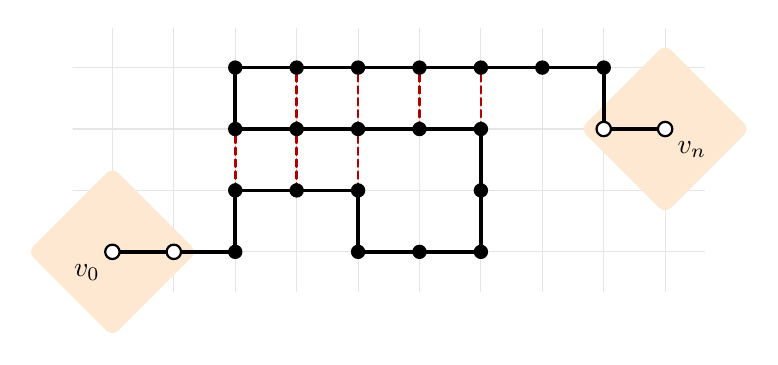
\begin{tikzpicture}[line cap=round]
\draw[black!10,step=0.78] (-0.5,-0.5) grid (7.52,2.84);
\fill[orange!18,rounded corners=3pt] (5.944,1.560) -- (7.020,2.636) -- (8.096,1.560) -- (7.020,0.484) -- cycle;
\fill[orange!18,rounded corners=3pt] (-1.076,0.000) -- (0.000,1.076) -- (1.076,0.000) -- (0.000,-1.076) -- cycle;
\draw[red!70!black,line width=1.0pt,dash pattern=on 2.5pt off 1.8pt] (1.560,0.780) -- (1.560,1.560);
\draw[red!70!black,line width=1.0pt,dash pattern=on 2.5pt off 1.8pt] (2.340,0.780) -- (2.340,1.560);
\draw[red!70!black,line width=1.0pt,dash pattern=on 2.5pt off 1.8pt] (3.120,0.780) -- (3.120,1.560);
\draw[red!70!black,line width=1.0pt,dash pattern=on 2.5pt off 1.8pt] (4.680,1.560) -- (4.680,2.340);
\draw[red!70!black,line width=1.0pt,dash pattern=on 2.5pt off 1.8pt] (3.900,1.560) -- (3.900,2.340);
\draw[red!70!black,line width=1.0pt,dash pattern=on 2.5pt off 1.8pt] (3.120,1.560) -- (3.120,2.340);
\draw[red!70!black,line width=1.0pt,dash pattern=on 2.5pt off 1.8pt] (2.340,1.560) -- (2.340,2.340);
\draw[black,line width=1.3pt] (0.000,0.000) -- (0.780,0.000);
\draw[black,line width=1.3pt] (0.780,0.000) -- (1.560,0.000);
\draw[black,line width=1.3pt] (1.560,0.000) -- (1.560,0.780);
\draw[black,line width=1.3pt] (1.560,0.780) -- (2.340,0.780);
\draw[black,line width=1.3pt] (2.340,0.780) -- (3.120,0.780);
\draw[black,line width=1.3pt] (3.120,0.780) -- (3.120,0.000);
\draw[black,line width=1.3pt] (3.120,0.000) -- (3.900,0.000);
\draw[black,line width=1.3pt] (3.900,0.000) -- (4.680,0.000);
\draw[black,line width=1.3pt] (4.680,0.000) -- (4.680,0.780);
\draw[black,line width=1.3pt] (4.680,0.780) -- (4.680,1.560);
\draw[black,line width=1.3pt] (4.680,1.560) -- (3.900,1.560);
\draw[black,line width=1.3pt] (3.900,1.560) -- (3.120,1.560);
\draw[black,line width=1.3pt] (3.120,1.560) -- (2.340,1.560);
\draw[black,line width=1.3pt] (2.340,1.560) -- (1.560,1.560);
\draw[black,line width=1.3pt] (1.560,1.560) -- (1.560,2.340);
\draw[black,line width=1.3pt] (1.560,2.340) -- (2.340,2.340);
\draw[black,line width=1.3pt] (2.340,2.340) -- (3.120,2.340);
\draw[black,line width=1.3pt] (3.120,2.340) -- (3.900,2.340);
\draw[black,line width=1.3pt] (3.900,2.340) -- (4.680,2.340);
\draw[black,line width=1.3pt] (4.680,2.340) -- (5.460,2.340);
\draw[black,line width=1.3pt] (5.460,2.340) -- (6.240,2.340);
\draw[black,line width=1.3pt] (6.240,2.340) -- (6.240,1.560);
\draw[black,line width=1.3pt] (6.240,1.560) -- (7.020,1.560);
\filldraw[fill=white,draw=black,line width=0.8pt] (0.000,0.000) circle (2.6pt);
\filldraw[fill=white,draw=black,line width=0.8pt] (0.780,0.000) circle (2.6pt);
\fill[black] (1.560,0.000) circle (2.6pt);
\fill[black] (1.560,0.780) circle (2.6pt);
\fill[black] (2.340,0.780) circle (2.6pt);
\fill[black] (3.120,0.780) circle (2.6pt);
\fill[black] (3.120,0.000) circle (2.6pt);
\fill[black] (3.900,0.000) circle (2.6pt);
\fill[black] (4.680,0.000) circle (2.6pt);
\fill[black] (4.680,0.780) circle (2.6pt);
\fill[black] (4.680,1.560) circle (2.6pt);
\fill[black] (3.900,1.560) circle (2.6pt);
\fill[black] (3.120,1.560) circle (2.6pt);
\fill[black] (2.340,1.560) circle (2.6pt);
\fill[black] (1.560,1.560) circle (2.6pt);
\fill[black] (1.560,2.340) circle (2.6pt);
\fill[black] (2.340,2.340) circle (2.6pt);
\fill[black] (3.120,2.340) circle (2.6pt);
\fill[black] (3.900,2.340) circle (2.6pt);
\fill[black] (4.680,2.340) circle (2.6pt);
\fill[black] (5.460,2.340) circle (2.6pt);
\fill[black] (6.240,2.340) circle (2.6pt);
\filldraw[fill=white,draw=black,line width=0.8pt] (6.240,1.560) circle (2.6pt);
\filldraw[fill=white,draw=black,line width=0.8pt] (7.020,1.560) circle (2.6pt);
\node[below left=1pt] at (0.000,0.000) {$v_0$};
\node[below right=1pt] at (7.020,1.560) {$v_n$};
\end{tikzpicture}
\caption{A path (solid) with its 7 chords (dashed), drawn in a plane for illustration; on $\T_L$ chords may also point out of the plane or across the periodic identification. Open circles are the uncharged vertices: the endpoints and their lattice neighbours on the path (shaded). Every induced bond at a charged vertex (black) has two interior endpoints, so the local inequalities (A1)--(A2) apply to it.}
\label{fig:path}
\end{figure}


\begin{proposition}[Cost of induced bonds]\label{prop:cost}
Let $u\ge u_0$ and let $(\alpha^{\rm P},\alpha^{\rm C},w,\theta,\gamma)$ be an allocation admissible for a table $\ell$ with $\ell_h\le\ell_h(u_0)$ for all $h$. Then for every even $L\ge8$ and every path $P=(v_0,\dots,v_n)$ on $\T_L$,
\begin{equation}\label{eq:cost}
 I(P,u)+\theta\,c(P)\ \ge\ \gamma\,(n-13)_+ +\sum_{i=1}^{n-2}w_{\tau_i}.
\end{equation}
\end{proposition}

\begin{proof}
Call a vertex of $P$ \emph{charged} if it is neither an endpoint $v_0,v_n$ nor a lattice neighbour of an endpoint lying in $V(P)$. There are at most $2+2\cdot6=14$ uncharged vertices, so at least $(n+1-14)_+=(n-13)_+$ charged ones. If $v$ is charged and $\{v,x\}\in D(P)$, then $x$ is not an endpoint, since otherwise $v$ would be a neighbour of an endpoint. Thus both ends of every induced bond touching a charged vertex are interior vertices of $P$.

Let $e=\{v,w\}\in D(P)$ have two interior endpoints. If $e=v_iv_{i+1}$ is a path bond, then $1\le i\le n-2$. The directions $d_-$ and $d_+$ of \cref{def:shape} point to occupied specified sites of the prism of $e$, so (A1) gives
\begin{equation}\label{eq:pathrow}
 \alpha^{\rm P}_{t_v(e)}+\alpha^{\rm P}_{t_w(e)}+w_{\tau_i}\le\ell_{h(e)}.
\end{equation}
If $e$ is a chord, each of $v,w$ is met by two path bonds different from $e$. Each hub thus has at least two occupied specified neighbours, and (A2) gives $\alpha^{\rm C}_{t_v(e)}+\alpha^{\rm C}_{t_w(e)}\le\ell_{h(e)}+\theta$.

Let $D^\circ$ be the set of induced bonds with two interior endpoints. By \cref{lem:prismbound}, the nonnegativity of $\ell$, and these two inequalities, each $e\in D^\circ$ satisfies $\ell_{h(e)}+\theta\one\{e\text{ chord}\}\ge w_e+\sum_{z}\alpha_{t_z(e)}^{\rm role(e)}$. Here $w_e=w_{\tau_i}$ if $e=v_iv_{i+1}$ is a path bond, $w_e=0$ for chords, and the sum runs over the \emph{charged} endpoints $z$ of $e$. Dropping the charge of an uncharged endpoint is allowed since all charges are nonnegative. Summing over $e\in D^\circ$,
\[
 I(P,u)+\theta\,c(P)\ \ge\ \sum_{e\in D^\circ}\Bigl(\ell_{h(e)}+\theta\one\{e\text{ chord}\}\Bigr)
 \ \ge\ \sum_{i=1}^{n-2}w_{\tau_i}+\sum_{z\text{ charged}}\ \sum_{e\in D(P),\,e\ni z}\alpha^{\mathrm{role}(e)}_{t_z(e)} .
\]
Every path bond $v_iv_{i+1}$ with $1\le i\le n-2$ belongs to $D^\circ$. For a charged vertex $z$ let $S\subset\{\pm e_1,\pm e_2,\pm e_3\}$ be the set of directions from $z$ to its neighbours in $V(P)$, and let $d_1,d_2$ be the directions of its two path bonds. The induced bonds at $z$ are exactly the bonds in the directions of $S$, and the half-edge in direction $d$ has type $t(d,S)$. By (A3) the inner sum is at least $\gamma$, which completes the proof.
\end{proof}

\begin{remark}
\Cref{prop:cost} involves no lift of $P$ to $\Z^3$ and no choice of orientation. It holds on every even torus with $L\ge8$, including paths that wind around the torus and chords across the periodic identification. The constant $13$ comes only from the endpoint neighbourhoods.
\end{remark}

\begin{remark}[Why a chord price is needed]\label{rem:hamilton}
A bound of the form $I(P,u)\ge\gamma'|P|-C$, valid for all paths with $C$ independent of $L$, forces $\gamma'\le f(K):=p(K,0)-\log2-3\log\cosh K$. Indeed, an even torus admits a Hamiltonian path $P$ (a ``snake'' visiting every site). For it $D(P)=E_L$, $|P|=V-1$ and $I(P,u)=\log\cE(u)=\log Z_L-V\log2-3V\log\cosh K$. Dividing by $V$ and letting $L\to\infty$ gives the claim. The quantity $f(K)$, the free energy of the high-temperature expansion per site, is small near $K_c$. In~\eqref{eq:cost} the snake has $c(P)\approx2V$, and most of its cost is paid by the chord price $\theta$. The chord price is in turn controlled by the chord moments of \cref{sec:counting}.
\end{remark}
